\documentclass[border=10pt]{standalone}
\usepackage{tikz}
\usetikzlibrary{shapes.geometric, arrows.meta, positioning, shadows, calc}

% Define colors
\definecolor{processblue}{RGB}{70, 130, 180}
\definecolor{arrowcolor}{RGB}{50, 50, 50}
\definecolor{annotationcolor}{RGB}{200, 100, 50}

% Define styles
\tikzset{
    process/.style={
        rectangle,
        rounded corners=5pt,
        minimum width=2.8cm,
        minimum height=1.2cm,
        text centered,
        draw=processblue,
        fill=processblue!20,
        font=\sffamily\small,
        drop shadow
    },
    arrow/.style={
        thick,
        ->,
        >=Stealth,
        color=arrowcolor
    },
    annotation/.style={
        font=\sffamily\footnotesize,
        color=annotationcolor,
        text centered
    }
}

\begin{document}
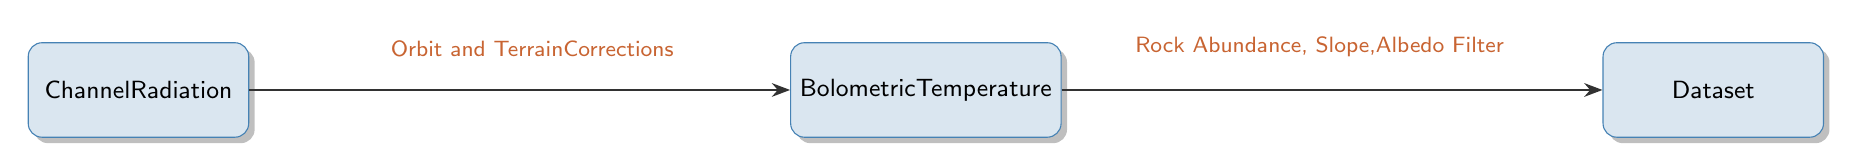
\begin{tikzpicture}[node distance=10.0cm]
    
    % Define main process nodes
    \node (channel) [process] {Channel\\Radiation};
    \node (bolometric) [process, right of=channel] {Bolometric\\Temperature};
    \node (dataset) [process, right of=bolometric] {Dataset};
    
    % Draw main arrows
    \draw [arrow] (channel) -- (bolometric);
    \draw [arrow] (bolometric) -- (dataset);
    
    % Add annotations above the arrows
    \node [annotation, above=0.3cm] at ($(channel)!0.5!(bolometric)$) {Orbit and Terrain\\Corrections};
    \node [annotation, above=0.3cm] at ($(bolometric)!0.5!(dataset)$) {Rock Abundance, Slope,\\Albedo Filter};
    
\end{tikzpicture}
\end{document}